%---------------------------------------------------
% کلاس سند: article برای اسناد متنی، با اندازه کاغذ A4 و فونت پایه 16
\documentclass[a4paper,16pt]{article}

% بسته‌های ریاضی برای معادلات و نمادهای پیشرفته
\usepackage{amsmath, amssymb, amstext}

% بسته رنگ برای استفاده از رنگ در متن یا محیط‌ها
\usepackage{xcolor}

% بسته گرافیک برای درج تصاویر
\usepackage{graphicx}

% تنظیمات حاشیه صفحه
\usepackage{geometry}

% بسته لینک‌دهی (هایپرلینک‌ها)
\usepackage{hyperref}

% بسته صفحه‌آرایی برای تنظیم هدر و فوتر
\usepackage{fancyhdr}


% بسته xepersian برای پشتیبانی از زبان فارسی با XeLaTeX
\usepackage{xepersian}

% تعیین فونت فارسی (فایل فونت باید موجود باشد یا در سیستم نصب باشد)
\settextfont{B Nazanin}

% تنظیم اندازه حاشیه‌ها از هر طرف برابر با 1 اینچ
\geometry{margin=1in}

% تنظیم سبک fancy برای سربرگ و پاورقی
\pagestyle{fancy}

% سمت چپ هدر: مشخص‌کننده سری تمرین و نام درس
\lhead{تمرین سری چهار درس فیزیک\lr{II }}

% وسط هدر: نام دانشکده
\chead{دانشکده فیزیک دانشگاه صنعتی خواجه نصیرالدین طوسی}

% سمت راست هدر: تاریخ روز به‌صورت خودکار
\rhead{\today}

% پایین صفحه: شماره صفحه
\cfoot{\thepage}

% شروع سند
\begin{document}
	
	% صفحه عنوان (بدون هدر و فوتر)
	\thispagestyle{empty}
	\begin{center}
		% لوگوی دانشگاه (باید فایل تصویر در مسیر پروژه باشد)
		
		
\includegraphics[width=0.5\textwidth]{../../../images/image-E_4/image-1.png} \\[10pt] 
		% عنوان سند
		\textbf{\LARGE عنوان:تمرین سری چهار }\\[20pt]
		
		% نیم‌سال تحصیلی
		\textbf{\LARGE نیم‌سال تحصیلی:4032 }\\[10pt]
		
		% نام مدرس درس
		\textbf{\Large مدرس: ‫دكتر‬ ‫رضا‬ ‫افضل‬ ‫زاده‬}\\[10pt]
		
		% مبحث تمرین 
		\textbf{\Large ‫مبحث ‬‫تمرين‪:‬‬ ‫پايان‬ ‫ترم‬ }\\[10pt]
		
		% مهلت تحویل تمرین
		\textbf{\Large ‫مهلت ‬‫تحويل‪:‬‬ ‫ارديبهشت‬۲۰ }
	\end{center}
	
	% صفحه جدید برای ادامه سند
	\newpage
	
	% ایجاد فهرست مطالب به‌صورت خودکار (براساس \section و \subsection و ...)
	\tableofcontents
	\newpage
	
	
	\section{سوال اول}
	
	میدان مغناطیسی اطراف یک سیم مستقیم با طول $L$ و جریان $I$ را در نقطه‌ای که فاصله آن از سیم برابر $r$ است، بدست آورید.
	
	\section{سوال دوم}
	
	یک هادی بلند و صلب که روی محور $x$ قرار دارد، جریان $I = 5.0~\mathrm{A}$ را در جهت منفی محور $x$ عبور می‌دهد.  
	میدان مغناطیسی $\vec{B}$ به صورت زیر داده شده است:  
	\[
	\vec{B} = 3.0~\hat{i} + 8.0 x^2~\hat{j} \quad 
	\]  
	نیروی وارد بر بخش $2.0~\mathrm{m}$ هادی که بین $x=1.0~\mathrm{m}$ تا $x=3.0~\mathrm{m}$ قرار دارد را به صورت برداری بدست آورید.
	
	\section{سوال سوم}
	
	یک الکترون در مسیری دایره‌ای به شعاع 
	\[
	r = 5.29 \times 10^{-11}~\mathrm{m}
	\]  
	با سرعت  
	\[
	v = 2.19 \times 10^{6}~\mathrm{m/s}
	\]  
	حرکت می‌کند. مسیر دایره‌ای را به صورت یک حلقه جریان با جریان ثابت برابر با نسبت اندازه بار الکترون به دوره حرکت در نظر بگیرید.  
	اگر این دایره در میدان مغناطیسی یکنواخت با بزرگی  
	\[
	B = 7.10 \times 10^{-3}~\mathrm{T}
	\]  
	قرار داشته باشد، بیشینه مقدار گشتاور مغناطیسی وارد بر حلقه را بیابید.
	\section{سوال چهارم}
	
	یک الکترون وارد یک سر سولنوید می‌شود. هنگامی که وارد میدان مغناطیسی یکنواخت داخل سولنوید می‌شود، سرعت آن 
	\[
	v = 800 m/s
	\]
	است و زاویه بردار سرعت آن با محور مرکزی سولنوید
	\[
	\theta = 30^\circ
	\]
	است. سولنوید جریان 
	\[
	I = 4.0A
	\] 
	را عبور می‌دهد و تعداد دورهای آن 
	\[
	N = 8000
	\] 
	در طول طول سولنوید است. تعداد دورهای الکترون در مسیر هلی‌کال داخل سولنوید تا زمانی که از انتهای مخالف آن خارج شود، چند است؟
	
	\section{سوال پنجم}
	
	یک سیم لوله تک‌لایه به طول \(L\) و شعاع سطح مقطع \(r\) دارد که بر روی آن \(N\) دور پیچیده شده است. اگر جریان الکتریکی \(I\) از سیم عبور کند، میدان مغناطیسی داخل سیم لوله (سولنوید) چقدر است؟
	
	\section{سوال ششم}
	

در شکل زیر، یک حلقه بسته جریان 
\[
i = 200~\text{\lr{mA}}
\] 
دارد. این حلقه شامل دو سیم مستقیم شعاعی و دو قوس دایره‌ای هم‌مرکز با شعاع‌های 
\[
r_1 = 2.00~\text{\lr{m}} \quad \text{و} \quad r_2 = 4.00~\text{\lr{m}}
\] 
است. زاویه بین دو سیم مستقیم 
\[
\theta = \frac{\pi}{4}~\text{\lr{rad}}
\] 
است.  

\begin{enumerate}
	\item[(الف)] مقدار اندازه میدان مغناطیسی خالص در مرکز انحنا \(P\) را بیابید.
	\item[(ب)] جهت آن (به داخل یا خارج صفحه) را تعیین کنید.
\end{enumerate}
	\begin{center}
	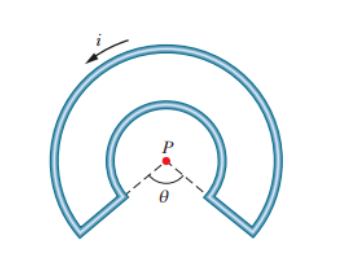
\includegraphics[width=0.5\textwidth]{../../../images/image-E_4/image-2.png} \\[10pt] 
\end{center}

	\section{سوال هفتم}
یک حلقه دایره‌ای به شعاع \(R_1 = 12~\text{\lr{cm}}\) حامل جریان \(I_1 = 15~\text{\lr{A}}\) است، و یک کویل تخت هم‌مرکز با شعاع \(R_2 = 0.82~\text{\lr{cm}}\)، \(N = 50\) دور و جریان \(I_2 = 1.3~\text{\lr{A}}\) دارد؛ صفحه حلقه عمود بر صفحه کویل است و میدان مغناطیسی حلقه در سراسر کویل یکنواخت فرض شده است.  


\begin{enumerate}
	\item[(الف)] مقدار میدان مغناطیسی تولید شده توسط حلقه در مرکز آن را بیابید.
	\item[(ب)] گشتاور وارد بر کویل به دلیل میدان حلقه چقدر است؟
\end{enumerate}

	\textbf{موفق باشید.}
\end{document}
